\documentclass[a4paper,12pt]{article}
\usepackage[utf8]{inputenc}
\usepackage{graphicx}
\usepackage{supertabular}
\usepackage[draft]{fixme} % \fxnote  \fxwarning  \fxerror  \fxfatal
\usepackage{subfigure}
\usepackage[final]{pdfpages} %To add the pdf page as frontpage
\usepackage{booktabs} %For tables, horizontal and splittable lines
\usepackage{rotating}
\usepackage[format=hang,font=small,labelfont=bf]{caption} %To create bold caption for tables and pictures
\setcounter{secnumdepth}{3} %Chap,Sec,Sub,Subsub
\usepackage{fullpage} % to use the whole page 
\usepackage{url}
\usepackage{setspace}  
\usepackage{hvfloat}
\usepackage{multicol}
\usepackage{color}
\doublespacing     % Inter lines space

%%%%%%%%%%%%%%% FANCY HDR Settings %%%%%%%%%%%%%%%%%%%%%%%%%%%%%%%%%%%%%%%%%%%
\usepackage{fancyhdr}
%\usepackage[head=30pt,foot=10pt]{geometry}
%\fancypagestyle{plain}
\pagestyle{fancy}
\setlength{\headheight}{15pt} %Set the height of the header
\topmargin=-20pt
\headsep = 35pt
\hoffset=+0.335in
\textwidth = 445pt
%\footheight = 10pt
\textheight = 680pt %715

\fancyheadoffset[L]{35pt} % gap between the header and the left side 
\fancyheadoffset[R]{10pt} % gap between the header and the left side 
%\fancyfootoffset[R]{10pt}
\footskip = 30pt
%\voffset=-3.5in

\fancyhead{} %Clear all headers
\fancyhead[R]{\slshape \rightmark} % To write the Subsection on the upper right[R] header side
%\fancyhead[LO]{\slshape \leftmark} % To write the Section on the upper Left header side
%\fancyhead[R]{\bfseries Enabling BPEL service execution on Java devices by means of model-to-text transformations} %To write the Thesis title on the upper Right header

\lhead{\setlength{\unitlength}{1mm}
\begin{picture}(0,0)
\put(0,0){\includegraphics[width=65mm]{pictures/Logo.png}}
\end{picture}}

\fancyfoot{} %Clear the footer
\fancyfoot[C]{\slshape \thepage}

%%%%%%%%%%%%%%%%%%%%%%%%%%%%%%%%%%%%%%%%%%%%%%%%%%%%%%%%%%%%
%%%%%%%%%%%%LST listings settings %%%%%%%%%%%%%%%%%%%%%%%%%%

% Basic settings of the listings package to "better" show the code 
\usepackage{listings}
% \lstset{ %
% language=Java,            % choose the language of the code
% basicstyle=\small,  % the size of the fonts that are used for the code
% basewidth={0.57em,0.57em},
% frame=trBL,			        % adds a frame around the code
% breaklines=true,		      % sets automatic line breaking
% showstringspaces=false,         % underline spaces within strings
% }
%%%%%%%%%%%%%%%%%%%%%%%%%%%%%%%%%%%
\definecolor{lightgray}{rgb}{.9,.9,.9}
\definecolor{darkgray}{rgb}{.4,.4,.4}
\definecolor{forestGreen}{RGB}{34,139,34}
\definecolor{orangeRed}{RGB}{255,69,0}
%%%%
\lstdefinelanguage{bpel}{
morekeywords=
{name,linkName,isolated,parallel,partnerLink,operation,portType,inputVariable,createInstance,variable,element,location,importType,partnerLinkType,myRole,messageType,properties,level,outputVariable,xmlns,version,encoding}
}

\lstdefinelanguage{xaml}{
morekeywords=
{TypeArguments,Name,Default,DisplayName,OperationName,ServiceContractName,Key,AddressUri,CanCreateInstance, LogName, Message, MessageNumber, Expression,CorrelationHandle,Request}
}

\lstdefinelanguage{xml}{
        basicstyle=\small,
        sensitive=false,
}
%%%
\lstdefinestyle{workflowStyle}{
language=XML,
alsolanguage=bpel,
alsolanguage=xaml,
%Formatting
basicstyle=\scriptsize,
sensitive=true,
showstringspaces=false,
numbers=left,
numberstyle=\tiny,
tabsize=4,
numbersep=3pt,
extendedchars=true,
xleftmargin=2em,
lineskip=1pt,
breaklines,
captionpos=t,
%Coloring
backgroundcolor=\color{lightgray},
morekeywords={BooleanExpression},
alsoletter={:,<,>,/,?},
morestring=[b]{"},
morecomment=[s]{<!--}{-->},keywordstyle=\color{forestGreen},
identifierstyle=\color{blue}\ttfamily,
stringstyle=\color{orangeRed}\ttfamily,
commentstyle=\color{forestGreen}\ttfamily
}
%%
\lstnewenvironment{workflow-code}[2]{
\lstset{caption=#1,label=#2,style=workflowStyle}
}{}
%%%%%%%%%%%%%%%%%%%%%%%%%%%%%%%%%%%%%%%%%%%%%%%%%%%%%%%%%%%%

% Last package to be imported
\usepackage[pdftex,linkbordercolor={0 0 1},bookmarks=true,hypertexnames=false,breaklinks=true]{hyperref}
\hypersetup{
pdfauthor = {Antonio Arfè},
pdftitle = {Enabling BPEL service execution on Java devices by means of model-to-text transformations},
pdfcreator = {LaTeX},
pdfproducer = {latex + ps2pdf}}

% Title Page
\title{Enabling BPEL service execution on Java devices by means of model-to-text transformations}
\author{Antonio Arf\`{e}}

% Commands for showing the most used acronyms
\newcommand{\nl}{\newline} 
\newcommand{\javarmi}{\textsc{Java RMI}}
\newcommand{\bpel}{\textsc{BPEL}}

% Make every section start in a new page
\let\stdsection\section  
\newcommand{\STE}[1]{\textcolor{red}{#1}}
\renewcommand\section{\newpage\stdsection}

%%%%%%%%%%%%%%%%%%%%%%%%%%%%%%% END SETTINGS %%%%%%%%%%%%%%%%%%
%%%%%%%%%%%%%%%%%%%%%%%%%%%%%%% BEGIN DOCUMENT %%%%%%%%%%%%%%%%

\begin{document}

% % % \thispagestyle{empty}
% % %  \begin{titlepage}
% % %  % - Begin of frontpage -
% % %  \fxnote{DRAFT version 1.0}
% % %  \begin{nopagebreak}
% % % 
% % % \begin{raggedleft}\advance\rightskip by-1cm
% % % \null\vskip 2.5cm
% % %      {\LARGE Antonio Arfè}
% % % \vskip 2cm
% % % {\fontsize{28}{32}\bfseries
% % % Enabling BPEL service execution on Java devices by means of model-to-text transformations fixme
% % % 
% % %  \par}
% % % \vskip 3cm
% % % {\Large Bachelor Thesis Project \ June 2012 - ---- 2012 \par} %fixme
% % % \vskip 3pt
% % % To be evaluated on fixme --$^{th}$ 2012  %fixme
% % % \end{raggedleft}
% % % \vfill
% % % \hbox{\vrule\vbox{\hrule
% % %                 \prevdepth0pt
% % %                 \vskip2pt
% % %                 \hbox{ Department of Computer Science }
% % %                 \hbox{ Federico II University}
% % %                 \hbox{ Via Claudio,}
% % %                 \hbox{ 80100 Naples }
% % %                 \hbox{ ITALY }
% % %                 \vskip2pt
% % %                 \vskip.5ex
% % %                 \vskip2pt
% % %                 \hrule}\vrule}
% % % 
% % %  \end{nopagebreak}
% % % 
% % %  \cleardoublepage
% % %  
% % % % - End of frontpage - begin of titlepage -
% % % \begin{nopagebreak}
% % % {\samepage
% % % \begin{tabular}{lr}
% % %         \parbox{14.5cm}{
% % %           {\LARGE Faculty of Engineering}
% % % 
% % %           {\small Federico II University}
% % %           \vspace{-0.3cm}\\
% % %         \hrule
% % %         \vspace{0.2cm}
% % %           {\bf Department of Computer Science}
% % %          }   & \hspace{-2.0cm} %\includegraphics[width=1.1cm]{picLogo.jpg} %fixme
% % % \end{tabular}
% % % %------------------------ with parbox at 7 cm
% % % \begin{tabular}{cc}
% % % \parbox{7cm}{
% % % \hspace{2cm}
% % % \begin{description}
% % % 
% % % \item {\bf TITLE:}
% % % 
% % % Enabling BPEL service execution on Java devices by means of model-to-text transformations
% % % 
% % % \end{description}
% % % 
% % % % ---------------------- Description with parbox at 8 cm
% % % \parbox{8cm}{
% % % 
% % % \begin{description}
% % %          \item {\bf PROJECT PERIOD:}\\
% % %            Bachelor Thesis, \\
% % %            %fixme Oct 1$^{st}$ 2012 -\\fixme 99$^{th}$ 2010\\
% % %             June 2012 -\\---- 2012\\
% % %            \hspace{4cm}
% % %          \item {\bf STUDENT:}\\
% % %            Antonio Arfè\\
% % %            \hspace{2cm}
% % %          \item {\bf SUPERVISORS:}\\
% % %            V. Vittorini, S. Marrone
% % % \end{description}
% % % }
% % % 
% % % %--------------------------------------------------------
% % % \begin{description}
% % %         \item {\bf NUMBER OF COPIES:} 4
% % %         \item {\bf REPORT PAGES:} \pageref{report_end}
% % %         \item {\bf APPENDIX PAGES:} 0
% % %         \item {\bf TOTAL PAGES:} \pageref{LastPage}
% % % \end{description}
% % % %--------------------------------------------------------
% % % \vfill } &
% % % \parbox{7cm}{
% % %   \vspace{.15cm}
% % %   \flushright
% % %   \fbox{
% % %     \parbox{6.5cm}{{\bf SYNOPSIS:}\vspace{0.5cm}
% % %      {\vfill{\small % Synopsis


	fixme.

	Lorem ipsum dolor sit amet, consectetur adipiscing elit. Sed lorem ante, porttitor vitae fringilla et, fermentum fermentum nisl. Nunc fringilla, dui viverra iaculis volutpat, augue massa ornare augue, ac sodales erat lectus non risus. Cras rutrum elit sit amet ligula interdum fermentum. Curabitur tincidunt, dui ut hendrerit mattis, massa turpis pretium lectus, eu sagittis turpis nibh id sem. Vestibulum consectetur sapien vel nisi vehicula eget dignissim diam malesuada. Cras consequat, tellus ut malesuada commodo, lacus libero adipiscing ligula, auctor laoreet ligula enim eu turpis. Aenean eget dui eget mauris facilisis faucibus. Curabitur quis metus est, a vulputate orci. Integer mollis metus ac purus condimentum

	fixme.
% % %      }}\vspace{0.3cm}
% % %      }
% % %   }
% % % }
% % % \end{tabular}
% % % }
% % % 
% % % %----------------------
% % % 
% % % \end{nopagebreak}
% % % \end{titlepage}

 
%\setcounter{page}{3}

\includepdf[pages=1-2]{frontespizio.pdf}
%pagina vuota se possibile

% Table of contents
\tableofcontents
\pagebreak

\section{Introduction}
%---Web Services Composition Contest
Today, the web is quickly expanding and new functionalities and applications, appearing day by day, are heavily increasing its potentialities and ease of use. Actually, one of the reasons why this growth is taking place is the possibility to connect and let communicate different existent applications, or better, \textit{services}.

%--- Today the web is going to composition of services
%--- This can be done with ad-hoc solutions or using paradigms to abstract the existent applications and show them as services in a standard way. SOC 
%--- The implementation of such services also needs an architectural infrastructure, comprehensive of tools, protocols and languages. SOA
%--- Once the services are put in place, several challenges arise, such as how to discover the services that are publicly available, how the providers can advertise them, how the services should integrate the usage of resources like files or databases, how they provide secure and private access to authorized users and, eventually, how to define the rules to compose and make collaborate the services together.   

%--- Focusing on the latter aspect, the composition of services can be achieved using two main approaches: Orchestration and Choreography.
%---  
 
% We intend the word \textit{service} as the one used by the UDDI Oasis consortium \cite{Uddi}, where services are self-contained and modular applications that have Internet-oriented and standard-based interfaces. The given definition of services tightly relates to some of the well known web standards used to implement Web Services (WSs) \cite{DiLorenzo08}.




%---Overview of the whole work---
\subsection{Overview of the thesis}

%Service Oriented Computing
\section{Service Oriented Computing}
\label{ServiceOrientedComputing}
This Section gives a brief overview of the Service Oriented domain and its components. We introduce in Section \ref{SOC&SOA} the paradigms to create service oriented infrastructures. Section \ref{WebServices} explains how services can be deployed using the web as media, namely, the Web Services. 
Later in Section \ref{WFManagement} we talk about Workflow management, introducing the terms of Orchestration and Choreography. Right after we dig into the technologies we will be working on throughout the whole project; we overview both BPEL in Section \ref{BPEL} and the remote calls enabled version of Java, Java RMI in Section \ref{JavaRMI}.   

\subsection{Services and composition, SOC and SOA}
\label{SOC&SOA}
During the years preceding the large spread of the Internet, companies used to create their own software systems, in order to obtain highly customized and specific services, rarely focused on the accessibility by external partners.
Today, with the necessity of exchanging information among different companies and businesses, and the push made by the large growth of the Internet, the focus has moved to the integration and the coordination of the existing softwares, namely, the integration of these systems over larger networks.
Defining a \textit{service} as a distributed application that exports a view of its functionalities  \cite{DiLorenzo08}, what is needed is the possibility to compose different services together.
For example, it might be useful to integrate a service (already available on a net), providing maps of a city's streets, with a web-based service listings telephone numbers of a given city zone, resulting in a new service showing telephone numbers on the map. %\fxnote{I might add a picture to better show the example here} FIXME
  
The \textit{Service Oriented Computing} (SOC) is the paradigm that attempts to wrap and adapt existing applications into new services, which should comply to three main requirements \cite{DiLorenzo08,Papazoglou03}:
\begin{itemize}
 \item technological independent: the service should be accessible via well known protocols and have a descriptions available on most of the IT environments.
 \item loosely coupled: the client and the provider of the service should not know each other's internal details.
 \item location transparent: clients should be able to get information and access to a service, irrespectively of their location. 
\end{itemize}
Eventually the SOC paradigm makes use of services as the atomic components for developing new applications (which, in turn, can be services too \cite{Papazoglou03}.


To apply the SOC paradigm, there is a need of an architecture infrastructure style, which gives the directives and guidelines to build such a service.  
The architectural infrastructure of the SOC is called \textit{Service Oriented Architecture} (SOA). 
The idea behind the SOA is to describe, publish and make available services (generally speaking, a combination of services) obtained from a preexistent set of applications. 
To achieve the results of making non-homogeneous applications, using different technologies and running on different platforms, work together, SOA makes use of standard interfaces and messaging protocols. This way each of the applications become an atomic, well defined and ready to be connected component. 
The SOA presents an architecture devised in three main components \cite{Pernici04} as shown in Fig. FIXME: toCreate\ref{fig:The Service Oriented Architecture (SOA)}:
a \textit{service provider}, which makes the service available. The service provider registers its service to the \textit{service registry}, which contains the list of available services and their descriptions. After the registration, the service provider waits for a client to request a service. The service registry can also apply custom access control policies or be entirely public. 
The \textit{service client} contacts the service registry to \textit{find} a service, it gets a contract and the address of the service, making a so called \textit{bind} with the provider. Then it \textit{uses} the service.


Being the realization of services usually based on the reuse of previously existent software, there are many ways to realize it and they can also be combined. For a company, the realization can go from the complete in-house realization to the outsourcing, to buy/leasing just parts of the needed services or to using wrappers/adapters to reuse the legacy software.
To conclude, from the SOA point of view, services are like black boxes, they can be invoked by service clients independently, without the need of knowing internal details. This makes clients and providers logically decoupled, the client only needs to know the name, the interface and the version of the service. Of course, provider, client and register must be able to use a common communication channel. 

\subsection{Web Services}
\label{WebServices}
We have seen that SOA is an architecture style aimed at the creation of services but it does not address the communication medium. \textit{Web Services} (WS) are an instance of a SOA where the communication channel is the web \cite{Pernici04}.
Web services implement the SOA through the application of three main technologies: \textit{SOAP}(Simple Object Access Protocol), \textit{WSDL}(Web Services Description Language) and \textit{UDDI}(Universal Description, Discovery and Integration).
On the picture of the SOA showed above, we can add these three components, as shown in Fig: (FIXME: to create)\ref{fig:SOA with webServ implement.}. The SOAP is the web protocol used to exchange messages among the parties. WSDL is the language used by the service provider to fully describe the offered service. At last, UDDI is used by the service registry to make a service easy to find, abstract its technology and make it accessible to the clients.
In the next paragraphs we have a brief look into these three technologies.

\subsubsection{WSDL (Web Services Description Language) }
\label{Wsdl}
WSDL is a language based on \textit{XML}(eXtensible Markup Language) and it permits to unambiguously describe a web service. For example, it can describe the input parameters a client must provide to use the service and the type of the result the client should expect. 
A WSDL description starts with a \textit{service} tag that identifies a group of related services. Each of the services is then described as following.
The first element is the \verb|port| which identifies the address and the protocol to access the service (e.g. from the IBM online examples,\cite{IBMWSDL} \\
\verb|<soap:address location="http://www.snowbo.../EndorsementSearch"/>|). \\
With \verb|portType|, there are given the specifics of any \verb|operation| that can be used by the client, for example, the input/output parameters or the error messages. The \verb|operation|s comply to one of 4 main patterns: the \verb|One_way| (client sending a message to the provider), the \verb|Request_response| (client sending a message and waiting for an answer form the provider), the \verb|Solicit_response| (Provider sending a message to the client and waiting for a response) and the \verb|Notification| (provider sending a message to the client).
The elements to define the messages and the types used by the service are \verb|message| and \verb|types|. The first specifies the structure of a message to be exchanged. The second, is used to define the atomic types (integer, string, etc.) or new custom types. 
The most important elements in a WSDL service description are summarized in Table \ref{tab:WSDLElements}.

Eventually, we can see that WSDL proposes a static picture of the service. It defines the address and the way to access the service, the operations and, for each of them, the input/output elements to be provided, but it has no notion of the order in which the operations should be called. For example, to access an online shop service, there might be the need to first perform a login operation, check the item availability and last, buy the item. Such a order or workflow, though, it is not addressed in a WSDL description. This workflow represents the dynamic behavior of a service and it is addressed by the \textit{WorkFlow Management Systems} (WfMS), discussed in the following Section.


% - Who is going to deal with the logic and flow of the composition? \nl 
% - Two main approaches: Orchestration and Choreography, where is the difference \cite{Peltz03} \nl
% - The concept of Workflow management \cite{Aalst98} (picture) and why BPEL is good at it.  \nl
% 
%%%%%%%%%%%%% WSDL TABLE of characteristics %%%%%%%%%%%%%%%%%%%%%%%%%%%%%%%%%%%%%%%%%%%%%%%%%%
\begin{table}
\caption{Basic WSDL elements and their description}
\label{tab:WSDLElements}
\begin{center}
\begin{tabular}{l p{11cm}}

						\toprule
						\addlinespace[0.2cm]
\textbf{WSDL element} 	& \textbf{Description}	\\ 
						\cmidrule(l){1-2}
\verb|port| 		& It identifies the address where the service is found and the protocol to access it 				\\[0,1cm]
\verb|portType| 	& It provides the description of the service, using the \textit{operation} element 				\\[0,1cm]
\verb|operation| 	& It is a basic functionality provided by the service. It lists the input and output messages that are exchanged, in one of the four communication patterns 														\\[0,1cm]
\verb|message| 		& It specifies the format of messages to be exchanged, e.g. the name and type of the variables they contain 	\\[0,1cm]
\verb|types|		& The atomic or user-defined data types in use  								\\[0,1cm]
\verb|binding|		& Given a portType, it describes how this is implemented in the specific protocol 				\\[0,1cm]
	 
						\addlinespace[0.2cm]
						\bottomrule
\end{tabular}
\end{center}
\end{table}
%%%%%%%%%%%%%%%%%%%%%%%%%%%%%%%%%%%%%%%%%%%%%%%%%%%%%%%%%%%%%%%%%%%%%%%%%%%%%%%%%%%%%%%%%%%%%%

\subsection{Wf management: Orchestration vs Choreography}
\label{WFManagement}
%This workflow is the dynamic behavior of a service and it is addressed by the \textit{WorkFlow Management Systems} (WfMS), discussed in the following Section.
The workflow description, needed to address the behavior of a web-service is controlled by the \textit{WorkFlow Management Systems} (WfMS). The activities are performed following an execution flow based on four main patterns \cite{Pernici04}: \verb|sequence|, \verb|AND_split|, \verb|OR_split|, \verb|join|. These patterns permit to create generic workflows which are scheduled depending on the availability of the resources.
Two approaches for the workflow management exist: Orchestration and Choreography \cite{Peltz03}. Although the two approaches might overlap, their aims differ (see Fig. \ref{fig:OrchAndChor}). 

\paragraph{Orchestration}
Orchestration describes the realization of an executable business where the overall control is given to one party. For example, we can show how a travel planner web service works (see Fig. \ref{fig:orchestration}). Once a client sets the dates and destination of his travel, the travel planner service (coordinator) contacts other three services to book a flight, a hotel and a car. The requests and responses to and from the orchestrated services, are dealt by the coordinator, which takes care of reporting the found travel information back to the client.
These three services can be separated modules, belonging to different companies and implemented with different technologies.
\paragraph{Choreography}
Choreography also describes the realization of an executable business process, but there is no party having overall control. Here each party collaborates and provides its part and role for the final result. Using the previous example (see Fig. \ref{fig:choreography}), we can notice that the stand alone services have no coordinator. They collaborate exchanging messages among each other. Eventually, choreography, takes care of the interactions among the services more than executing a process from one party's perspective.

\subsubsection{Workflow Management for Web Services}
Among the workflow management systems, there are: FIXME Introduce BPEL and describe it in the next Subsection.


%%%%%%%%%%%%%%%%%FIGURE %%%%%%%%%%%%%%%%%%%%%%%%%%%%%%%%%%55 
 \begin{figure}
\centering
\subfigure[Service orchestration. The travel planner service coordinates the activities of the car rental, flight booking and hotel booking services. ]{
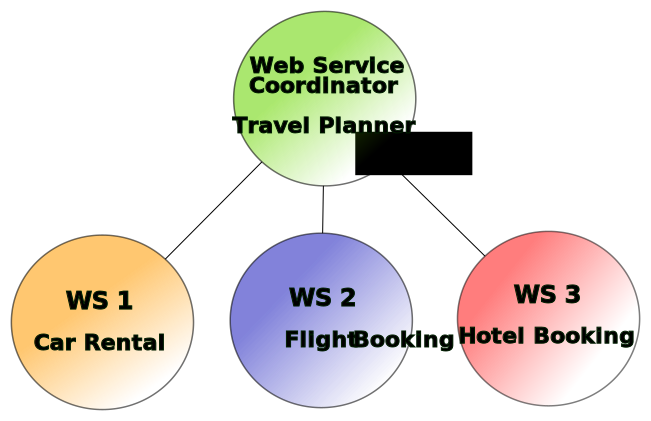
\includegraphics[scale=0.32]{pictures/FigOrchestration}
\label{fig:orchestration}
}
\hspace{2mm}
\subfigure[Service choreography. The services here collaborate to realize the main objective.]{
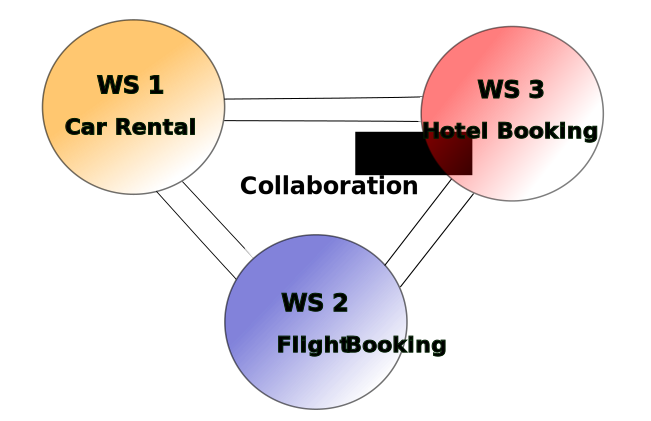
\includegraphics[scale=0.32]{pictures/FigChoreography}
\label{fig:choreography}
}
\caption{Example of service orchestration versus service choreography}
\label{fig:OrchAndChor}
\end{figure} 
%%%%%%%%%%%%%%%%%%%%%%%%%%%%%%%%%%%%%%%%%%%%%%%%%%%%%%%%%%%%%%%

%\subsection{BPEL} FIXME: review!
% Literature review: BPEL - the overview
% Author: František Kobzík

\subsection{BPEL - The Overview} \label{BPEL}

%FIXME-ANT 4-12: Franti I don't know where to place these citations
%\cite{BPEL-introduction}
%\cite{BPEL-ecplise}

%MODIFIED by Anto 4/12
Today's companies want to exchange data effectively and get communication and business flow as fast as possible, in order to save time, and thus money. They want to automate their business processes and speed up the information exchange. BPEL is a standard that can help them to achieve this goal.
BPEL (which stands for Business Process Execution Language) is an XML standard for describing and defining business processes and hereby standardize the format of information's exchange between different softwares. 

BPEL was initially developed by IBM and Microsoft. Its first version (1.0) was released in 2002 by these companies and BEA. Developers wanted to merge IBM's WSFL and Microsoft's XLANG. Both WSFL and XLANG have the same purpose - to combine web services in supporting business processes. During the following year, other companies (Siebel Systems and SAP) joined the development of BPEL and one year later they released version 1.1 together. After this, BPEL was passed to the OASIS nonprofit consortium. In 2007 Web Services BPEL (WS-BPEL) version 2.0 standard was released. During the year 2005 OASIS announced development of extension of WS-BPEL called BPEL4People, including the human interaction in BPEL processes.
\cite{BPELonWikipedia}

%MODIFIED by Anto 4/12 
\paragraph{BPEL Architecture example} \label{BPELarchitecture}
This paragraph contains a brief example of a simple BPEL server and its description. Note that this is not a general case since BPEL specification does not include any description of the architecture of a BPEL system and therefore this part serves for a reader to get an idea of how BPEL process works (see Figure \ref{BPELprocess}).  
In a typical, scenario BPEL process is run on some BPEL engine which is accessible through web services (which among other things contributes to BPEL Architecture platform and operating system independence). After deploying the process, the engine waits for a request (WSDL messages) from clients (which can be for example another BPEL server or a web interface). After the request is received, the BPEL engine creates an instance of a BPEL process and runs it. When running, the process can further interact with the client and also with different BPEL servers. At the end of the operation the result is sent to the client and the process is destroyed in the server.

\subsubsection{BPEL Activities} 
\label{BPELActivities}

In a BPEL process, activities are used to define the process logic. Activities are divided into two classes: basic and structured. 

\begin{enumerate}
\item Basic activities are those which describe elementary steps of the process behavior. The following is a list of the most important ones:
	\begin{itemize}
	\item \verb|<invoke>|
	\item \verb|<receive>|
	\item \verb|<reply>|
	\item \verb|<assign>|
	\item \verb|<throw>|
	\end{itemize}

\item Structured activities encode control-flow logic, and can contain other basic and/or structured activities recursively. The most important are listed below:
	\begin{itemize}
	\item \verb|<sequence>|
	\item \verb|<flow>|
	\item \verb|<if>|, \verb|<while>|, \verb|<repeatUntil>|  
	\item \verb|<pick>|
  \end{itemize}
\end{enumerate}

%MODIFIED by Anto 4/12 
\subsubsection{BPEL Communication}
\label{BPELCommunication}
BPEL processes need to communicate with each other and for this purpose they usually use the combination of a description language, WSDL, and a protocol, SOAP. WSDL stands for Web Services Description Language and is used to define the interfaces between communicating processes. It means that WSDL determines the format of messages, their data types and types of ports used for transmitting messages \footnote{each port has a particular type(s) assigned and therefore it can receive/send messages of this type(s) only} Whereas WSDL defines the interface between processes, SOAP works on lower level and is used for transmitting the data. There is a detailed description of SOAP in section \ref{Soap} of this document.

\begin{figure}
\begin{center}
\includegraphics[width=125mm]{pictures/image-BPEL.pdf}
\caption{Execution of a simple BPEL Process}
\label{BPELprocess}
\end{center}
\end{figure}

\subsubsection{Technologies and protocols used by BPEL}
As mentioned before, BPEL uses WSDL to define process interface and SOAP for message transmitting. On lower levels XML Schema is used for defining the type of XML documents which are sent and received. On the lowest level XML is used for data encapsulation. This can also vary from implementation to implementation. Some engines (i.e. Oracle BPEL Process Manager) allow to communicate with each other using Java RMI instead of SOAP. WS-BPEL 2.0 standard adds some new technologies like XPath for accessing data in complex variables and XSLT operations for transforming them.
\cite{OraBPELRMIInvocation}

%FIXME-franta I don't know where is the following paragraph from, because I didn't write it and I can't find anything about it in the existing references...
\label{BPELfiles}
BPEL is based on XML language. As a programming language it has three basic components: the programming logic, the data types and the input/output (I/O). They are divided in three files written in three languages: BPEL, XML Schema definition and WSDL. 
The BPEL file contains the "orchestration" of the system. It specifies an executable process that involves message exchanges between the various processes composing the system. The XML Schema file is used to define the types used in the program. The WSDL file defines the Web Service from an "abstract" point of view describing all the operations for each process participating in the business service.
Table \ref{BPELfilesTable} summarizes the functionalities of the three files composing a BPEL process.

%%%%%%%    Table %%%%%%%%%%%%%%%%%%%%%%%%%%%%%%%%%%%%%%%%%%%%%%
\begin{table}[h!]
\begin{center}
\begin{tabular}{l l l}
						\toprule
						\addlinespace[0.2cm]
\textbf{Basic Components} 	& \textbf{Language} 	& \textbf{File extension} 	\\ 
						\cmidrule(l){1-3}
Programming Logic 		& BPEL			& .bpel 			\\[0,1cm]
Data Types 			& XSD (XML Schema) 	& .xsd 				\\[0,1cm]
Input/Output 			& WSDL 			& .wsdl 			\\[0,1cm]
						\addlinespace[0.2cm]
						\bottomrule
\end{tabular}
\end{center}
\caption{BPEL files' functionalities}
\label{BPELfilesTable}
\end{table}
%%%%%%%%%%%%%%%%%%%%%%%%%%%%%%%%%%%%%%%%%%%%%%%%%%%%%%%%%%%%%%

%FIXME-ANT: 4/12 I added some ``escape from engine'' lines, but I'm not sure about this paragraph.
\paragraph{BPEL Engines}
Table \ref{BPELengines} represents several common BPEL engines developed by various companies. In this document we won't go deep into the engines' details because we will concentrate more on the BPEL process, its orchestration and its functionalities. Of course, sometimes it is not possible to explain BPEL concepts without basic knowledge about the engines. Thus, brief explanation will be provided in further sections when necessary.
\cite{BPELenginesComparisonOnWikipedia}


%%%%%%%%% Table %%%%%%%%%%%%%%%%%%%%%%%%%%%%%%%%%%%%%%%%%%%%%%%%%%%%%%%%%%%
\begin{table}
\begin{center}
\begin{tabular}{l l l}  %\begin{tabular}{|p{5.5cm}|p{3cm}|p{2.5cm}|}
						\toprule
						\addlinespace[0.2cm]
{\bf Name of BPEL Engine} 	& {\bf Supported BPEL Version} 	& {\bf License} 	\\
						\cmidrule(l){1-3}
ActiveBPEL         		& BPEL4WS 1.1, WS-BPEL 2.0 	& GPL and commercial 	\\[0,1cm]
Apache ODE         		& WS-BPEL 2.0 			& Apache license	\\[0,1cm]
jBMP (jBoss)         		& WS-BPEL 2.0 			& LGPL			\\[0,1cm]
Open ESB (Oracle)		& WS-BPEL 2.0 			& Open Source		\\[0,1cm] 
Oracle BPEL Process Manager   	& BPEL4WS 2.0 			& commercial		\\[0,1cm]
WebSphere Process Server (IBM)	& WS-BPEL 2.0			& commercial		\\[0,1cm]
						\addlinespace[0.2cm]
						\bottomrule
\end{tabular}
\end{center}
\caption{List of BPEL engines}
\label{BPELengines}
\end{table}
%%%%%%%%%%%%%%%%%%%%%%%%%%%%%%%%%%%%%%%%%%%%%%%%%%%%%%%%%%%%%%%%%%%%%%%%%%%

%\subsection{Java RMI} FIXME: review!
% Literature review: Summary of Java RMI
% Author: Pierre

\subsection{Java RMI} \label{JavaRMI}   

\textit{Java RMI}, as the name suggests, is an extension of the Java object model, that provides support for distributed objects in the Java language. The remote method calls are done using the same syntax as for local calls, the only difference is that the object making the invocation is aware that its target is remote, as it must handle \textit{RemoteExceptions}. On the other hand, the implementer of a remote object is aware that it is remote because it must implement the \textit{Remote} interface. In order to fill this section we used the Java RMI technology overview \cite{RMI-sun} and the tutorial from the SUN website \cite{RMI-client-sun} and \cite{RMI-overview-sun}.

\paragraph{Remote Interfaces in \textit{Java RMI}}

Remote interfaces are defined by extending an interface called \textit{Remote}, provided in the \textit{java.rmi} package. The remote methods must throw a \textit{RemoteException} in addition to any application specific extension. A remote interface can receive both ordinary and remote objects as arguments, which is also true for its results.

\paragraph{Parameter and result passing}

The arguments of a method are described as \textit{input}, whereas the result is a single \textit{output} parameter. Any object implementing the \textit{serializable} interface (thus being serializable) can be passed as an \textit{input} or \textit{output} in Java RMI.
When the type of a parameter or result value is defined as a remote interface, the corresponding argument or result is always passed as a remote object reference. On the other hand, when a remote object reference is received, it can be used to make RMI calls on the remote object it refers to.
All serializable non-remote objects are copied and passed by value. This way, a new object can be changed locally, possibly causing its state to differ from the one of the original object.

\paragraph{Downloading of classes}

Thanks to Java's virtual machine, classes can easily be transferred from one system to another. This feature is quite useful when placed in the context of distributed objects communicating through remote invocations. If a recipient does not possess the class of an object that has been send to it, the fitting code is downloaded automatically. This allows clients and servers to make transparent use of instances of new classes whenever they are added. Furthermore, there is no need for users to keep the same set of classes in their working environment.

\paragraph{RMI registry}

RMI registry is the middleware in charge of the binding tasks in \textit{Java RMI}. It has to be run on every server hosting remote objects. The RMI registry is actually in charge of maintaining a mapping table associating symbolic object names with remote objects hosted on this computer. It is accessed by methods of the \textit{Naming} class :
\begin{description}
\item[static void 	bind(String name, Remote obj)]
    Binds the specified name to a remote object.
\item[static String[] 	list(String name)]
    Returns an array of the names bound in the registry.
\item[static Remote 	lookup(String name)]
    Returns a reference, a stub, for the remote object associated with the specified name.
\item[static void 	rebind(String name, Remote obj)]
    Rebinds the specified name to a new remote object.
\item[static void 	unbind(String name)]
    Destroys the binding for the specified name that is associated with a remote object.
\end{description}
These methods take a string formatted in the following way as an argument:
\verb|//computerName:port/objectName|
where \textit{computerName} and \textit{port} refer to the location of the RMI registry.
\cite{DS-book}

% New part added by Antonio
% FIXME - I don't know the source of the following text. I need it for citations... I had a look to the "cite" at the beginning of this section, but no source of them fits to it..... :(

\subsubsection{Java RMI Architecture} 
\label{JavaRMIArchitecture}

\paragraph{Interfaces}
\label{JavaRMIinterfaces}
The RMI architecture is based on one important principle: the definition of a behavior and its implementation are separate concepts and their code run on separate JVMs. Moreover, the behavior is described in a Java Interface whereas the implementation is coded in a class \cite{RMI-art5}.
The Java Interface, containing the behavior, runs on the server. There are two implementations of this interface:
\begin{itemize}
	\item On the Server: Behavior's implementation class
	\item On the Client: Proxy class object
\end{itemize}

The client makes method calls directly on the proxy class object, then the proxy sends the request to the server's JVM which contacts the implementation. Any return values are sent back the other way around.

\paragraph{RMI architecture layers}
\label{RMIarchitectureLayers}

\begin{figure}
\begin{center}
\includegraphics[angle=90, scale=0.65]{pictures/rmi.pdf}
\caption{The layers of RMI}
\label{RMIlayers}
\end{center}
\end{figure}

The RMI implementation is built by three abstract layers shown on Figure \ref{RMIlayers}:

\begin{enumerate}
\item Stub/Skeleton
\item Remote Object Reference
\item Transport Layer
\end{enumerate}

\subparagraph{The Stub and Skeleton layer}
From the client's point of view the Stub object is a proxy which receives all requests directed to the server's service. The Skeleton, on the server side, does almost the same: receives the request from the Stub and passes it to the "real" object containing the method's implementation. Stub and Skeleton don't make any calculation or change on parameters, they just contain the code to communicate to each other. This avoids having to write the implementation of the "communication channel" directly in the client or server Java file. This is why the method's calls look like so similar to local calls. From the JDK 1.2 the Skeleton is not used anymore.
\subparagraph{The Remote Object Reference layer}
The Remote Object Reference layer provides a \verb|RemoteRef| object that represents the link, for the stub, to the class containing the implementation on the server. 
\subparagraph{The transport layer}
The transport layer makes the connection between JVMs and it uses the TCP/IP protocol. Even if two JVMs, containing two different services, are running on the same physical machine, they will connect through the TCP/IP protocol stack. 

%**********************************************************************************

\subsubsection{Java RMI: The Internal Mechanism}
\label{JavaRMIinternalMechanism}

This section concretely explains how Java RMI works and how it can 
help programmers in the writing of the network related code in their programs.

A typical scenario could be: a client wants to execute a method on the server which is on another machine. We will explain why the programmer does not have to write the network and sockets code with Java RMI.

We know that for the service interface on the server, there are two implementations with the same methods: the Stub on the client side and the real object implementing the behavior on the server side. In particular the client uses the stub to call all the methods the same way it would call them on the server. The only difference with a local call is that the stub does not contain the concrete implementation of the required function, it just contains the network-related code to create the communication channel with the server's real implementation \cite{RMI-art4}.
%Thus, from the JDK 1.2, there will be three classes: the client, the stub and the server's real implementation.     
%Client<--->stub<--->[NETWORK]<--->Server_real_implementation.

\paragraph{Socket-Level Details}
\label{SocketLevelDetails}

The following is the list of steps executed by a Java RMI program for each method's call:
\begin{enumerate}
\item The server object listens on an anonymous port on the server machine. The port is chosen at runtime by the JVM or the OS.
\item The client does not know the particular port on the server where the object is listening. It calls the method locally on the stub.
\item The stub creates a TCP/IP communication channel between client and server and it works in 5 steps: 
	\begin{itemize}
	\item The client connects to the server's listening port (see the Bootstrap problem paragraph to understand how the          Stub can know the server's address and port).
  \item The server, waiting for a client's request, accepts the incoming connection and creates a new socket just to 				  handle this single connection.
  \item The server will continue to use the old listening port to wait for other incoming requests.
  \item The communication between client and server takes place using the newly created socket on the server.
  \item They communicate and exchange parameters and results with an agreed-upon protocol. The protocol can be                 \textit{JRMP} (Java Remote Method Protocol) or CORBA-compatible \textit{RMI-IIOP} (Internet Inter-ORB                  Protocol).
	\end{itemize}
\item The method is executed on the server's real implemented object and the result is sent back to the stub.
\item The Stub returns the result back to the client object as if the stub had executed the method locally.
\end{enumerate}

\paragraph{Bootstrap problem}
\label{BootstrapProblem}
In point 2 of paragraph \ref{SocketLevelDetails} we did not explain how the stub on the client side can know the anonymous port where the object is listening on the server. The client has to know at least the IP address of the server machine where the service is available; thus the only problem for the client side is to get the anonymous port.
The RMI registry is used for this purpose: it stays on the server and keeps the correspondences between the name of the service and its address, in a table.
The Registry keeps pairs of $<$public\_name, Stub\_object$>$ in a hashmap, where:
\begin{description}
\item [public\_name] is the name attributed by the server to the implemented object.
\item [Stub\_object] is an instance of the Stub object containing also the address of the anonymous port. 
\end{description}

The following list explains how the Bootstrap problem is solved in Java RMI:
\begin{enumerate}
\item The RMI registry is also a Remote Object and listens on a well-known port on the server machine, by default the 1099.
\item The server creates an object (we call it the \textit{ServiceObject}) listening on an anonymous port.
\item The server automatically creates a \textit{Stub\_ServiceObject} of the new \textit{ServiceObject}
\item When \textit{rebind(String name, Remote obj)} is called on the server side, it passes a Remote Object Reference of the \textit{ServiceObject}, containing the exact port address, as the second parameter. The RMI registry Naming class constructs a new stub object in the registry by copying the already existing \textit{Stub\_ServiceObject} on the server machine and by adding the Remote Object Reference to it.
\item Now there is a pair $<$public\_name, Stub\_object$>$ in the RMI registry containing the name of the service and a Stub object also containing the "real" address of the \textit{ServiceObject} on the server.
\item When the client executes Naming.lookup(public\_name) (e.g \\ Naming.lookup("rmi://Server\_IP\_address:1099/calc") ) it passes the public name as the parameter to the RMI registry on the server. 
\item The RMI registry returns the stored \textit{Stub\_object} object back to the client. Now, the client gets a stub object that knows about the server's host name and port to which the server listens.
\item Now the client can just invoke the \textit{Stub\_object}'s method which will call the same method of the \textit{ServiceObject} on the server.
\end{enumerate}

After all these steps the client and the server don't need the RMI registry anymore. Actually, instead of the Registry, programmers could use different solutions to let the client know about the server's port where the \textit{ServiceObject} is listening, but we will not go into the details of these techniques. 
About the stub, we could say that it is the core of the RMI mechanism. After the Bootstrap it permits programmers to get rid of the communication protocol between client and server and to easily make remote calls like local calls.

%- Overview, features. - Why? it can run everywhere, lightweight scenarios.
%\subsection{Jet}
%\subsection{EMF and Open Architecture Ware (Eclipse)}
%\subsection{other...} 


% %---Where the problem is---
% \subsection{BPEL, its drawbacks and the use of WSs in a lightweight scenario}
% %\subsection{The drawbacks of using BPEL (BPEL and its possible drawbacks)}
% - BPEL, the de-facto standard concerning web services composition. \nl
% - Overview and brief review\nl
% - What do we use of it, the whole language or just a part? \nl %Questo dove andrà??
% - Problems: It works over Distributed Systems, engine powerful but heavy, DS not always available. \nl %i problemi che ha in generale e quelli specifici al nostro caso
% 
% %---Why we face the problem and which is the possible solution (and aim of the work)---
% %\subsection{Web Services Composition in lightweight scenario}
% - That's our question \nl
% - Sometimes we might need services composition working in less powerful environments than distributed systems. Examples? \nl
% - But we don't want to create a new application from scratch neither...(change hardware?).  \nl




%---Introduction to the MDA and how it basically works
\section{Model Driven Approaches}
\label{ModelDrivenApproaches}

\subsection{The Model Driven Architecture (MDA)}
\label{MDA}

\subsubsection{Model Driven Engineering}
\label{MDE}
\subsubsection{Model to Text transformation (M2T)}
\label{M2T}
\subsubsection{Acceleo}
\label{Accelelo}

%- What it is \nl
%- Why we use it, why is good (because it is generic, Architecture independent, Reuse)  \nl
%- How we use it: From BPEL processes to Java RMI processes \nl

 
%- %\subsection{MDE: Model Driven Engineering}
% Model-driven engineering (MDE) is a software development methodology which focuses on creating models rather than computing and algorithmic concepts usually addressed in the classical programming approaches.
% This discipline attempts an abstraction of the benefits and the features provided by the Software Engineering \cite{Marrone}, usually creating a domain specific framework for implementing new systems, based on well known and tested concepts, obtained through a careful and detailled analysis of the domain and its actors.
% The best known MDE initiative is the Object Management Group (OMG) initiative Model-Driven Architecture (MDA), which is a registered trademark of OMG \cite{MDE}.
% How we do it: Why we do it, What particular method we use and what logic architecture we use
\section{The methodological approach}
\label{MethodApproach}
%---What methodology we used---

We analyze the possibility of automatically transform a BPEL written process in a Java executable routine, with minimum ad-hoc developer’s intervention. Our final objective is to show the feasibility of a semi-automated transformation from a small business process orchestrated with BPEL to the Java language.
This section describes the methodological approach we undertaken to realize our objective. The steps are summarized as following:

\begin{itemize}
 \item We identify the subset of BPEL instructions suitable for a proof of concept of the transformation.
 \item Select a BPEL meta-model that covers the chosen subset of instructions.
 \item Individuate a BPEL workflow pattern to work on
 \item Choose a model driven methodology that allows us to manipulate  the BPEL input model (M2M, M2T) and that is compatible with a ready to run code output.
\end{itemize} 

Once these steps have been accomplished, we focus on providing more details on how we carry out the transformation. The main points are:
\textbf{DA SCRIVERE NELLA SEZIONE DETAILED ARCHITECTURE ? }
\begin{itemize}
 \item Provide a correspondence from BPEL constructs to Java concepts
 \item Design the structure of the output application.
 \item Define the essential skeleton of Java classes necessary to create a runnable BPEL process
 \item In the templates, describe how to use and where the dynamic information taken from the BPEL input model has to be placed.
 \item Plan where and how, in the architecture, the developer intervention has to take place.
 \item \textbf{Issues encountered and proposed solutions  ? }
\end{itemize} 
 
 To mention later: \\
 StubPartnerLinks, code to be input by the user, static code, the problem with the WSDL file

\subsection{The BPEL subset of instructions}
\label{Sec:BPELsubset}
The BPEL standard (see Section \ref{BPEL} for more details) has a wide variety of elements and instructions aimed at managing the possible workflow patterns obtainable during a services orchestration. Moreover, BPEL does not restrict the number of services that can participate to the orchestration neither the type and the quantity of interactions among them.
For these reason, we focus our attention on a subset of the whole BPEL language, both to restrain the complexity and to fit the time frame of the project.
\subsubsection{The activities subset}
We decided to restrict the BPEL activities to a subset containing the following constructs divided in four groups:
\begin{center}
\begin{supertabular}{p{0.4\textwidth}p{0.4\textwidth}}

1. Basic activities: 			& 2. Structured activities:		\\
\begin{itemize}
	\item \verb|<invoke>|
	\item \verb|<receive>|
	\item \verb|<reply>|
	\item \verb|<assign>|
	\end{itemize} 			&

					    \begin{itemize}
					      \item \verb|<sequence>|
					     \end{itemize}			\\
					     
3. Elementary operations: 		& 4. Static descriptive elements:	\\					
\begin{itemize}
	\item \verb|<copy>|
	\item \verb|<from>|
	\item \verb|<to>|
  \end{itemize} &

					    \begin{itemize}
					      \item \verb|<process>|
					      \item \verb|<partnerLink>|
					      \item \verb|<variable>|
					      \item \verb|<expression>|
					    \end{itemize}\\
\end{supertabular}
\end{center}

These elements allow the creation of simple BPEL processes, where the activities such as: invoking a service or waiting for a reply, happen as a sequence, one after the other. Although this limits the expressive potentiality of BPEL, it fits our need of focusing on proving the feasibility of an automated transformation from BPEL to Java without having to deal with the complexity of the whole language.
In Figure \ref{fig:SubSetBPEL} the BPEL subset of elements used for this project is depicted.

\begin{figure}
  \begin{center}
    \includegraphics[scale=0.67,angle=90]{pictures/SubSetBpel2.png}
    \caption{The BPEL subset in its ecore model representation}
    \label{fig:SubSetBPEL}
  \end{center}
\end{figure} 

\subsubsection{The meta-model for the BPEL subset}
\label{Sec:DesignBpelSubset}
To permit the parameterization of the BPEL process input model, we need a meta-model describing our subset. The Eclipse Modeling Framework (see Section \ref{EMF}) provides a meta-model written in ecore for the whole BPEL language; we use only the subset elements of this ecore meta-model.
\subsubsection{The BPEL workflow pattern to focus on}
\label{sec:DesignBPELPattern}
The BPEL language with its wide range of activities and operation, gives the possibility to orchestrate many kind of workflow patterns among the participant services. We concentrate our attention on a process having the following participants:
\begin{itemize}
 \item one partner link representing a client
 \item one partner link describing a web-service
\end{itemize}
and on a simple workflow pattern that concerns the activities shown in Figure: \ref{fig:BPELWorkflowPattern}\footnote{This Figure has been realized using the BPEL designer facilities of Eclipse. Yet not a standard, as the Oasis consortium has not released a graphical standard, many vendors provide very similar graphical notations}. The pattern shown in the Figure includes the following steps:
\begin{enumerate}
 \item the process waits for a client to connect and provide an input
\item reception of the input and its assignation to a variable to forward to the web-service.
\item web-service invocation
\item reception of the web-service's reply and assignation to a variable to be forwarded back to the client
\item final response sent back to the client
\end{enumerate}


\begin{figure}
  \begin{center}
    \includegraphics[scale=0.8]{pictures/BPELSimpleProcess.png}
    \caption{The BPEL workflow pattern we focus on}
    \label{fig:BPELWorkflowPattern}
  \end{center}
\end{figure} 
% %\lipsum[2]
% \hvFloat[
%  floatPos=!htb,
%  capWidth=h,
%  capPos=r,
%  capAngle=90,
%  objectAngle=90,
%  capVPos=c,
%  objectPos=c]{figure}{\includegraphics[scale=0.7]{pictures/SubSetBpel2.png}}%
% {Caption vertically centered right beside the float with a caption
% width of figure width and 
% \texttt{floatcapsep=5pt} (the default)}{fig:label}


\begin{figure}
  \begin{center}
    \includegraphics[scale=0.9]{pictures/TransformationApproach.png}
    \caption{The methodological transformation approach}
    \label{fig:TransformationApproach}
  \end{center}
\end{figure}

%----------------------------------------------------


% \begin{multicols}{2}
% \begin{enumerate}
%     \item Basic activities:
%     \begin{itemize}
% 	\item \verb|<invoke>|
% 	\item \verb|<receive>|
% 	\item \verb|<reply>|
% 	\item \verb|<assign>|
% 	\end{itemize}
%     \item Structured activities: 
%     \begin{itemize}
% 	\item \verb|<sequence>|
%     \end{itemize}
%     \item  Elementary operations:
%     \begin{itemize}
% 	\item \verb|<copy>|
% 	\item \verb|<from>|
% 	\item \verb|<to>|
%     \end{itemize}
%     \item Static descriptive elements:
%     \begin{itemize}
% 	\item \verb|<process>|
% 	\item \verb|<partnerLink>|
% 	\item \verb|<variable>|
% 	\item \verb|<expression>|
%     \end{itemize}
% \end{enumerate}
% \end{multicols}
\section{Detailed Architecture}
\label{DetailedArchitecture}
In this Section we introduce the tool we use to realize the chosen methodological approach. In addition, we describe the constraints under which we carry out the transformation, such as the use of a BPEL subset and the specification of a workflow pattern.
Later in this Section, we introduce the design ideas of our transformation and the general architecture we adopted.\\

FIXME: TO REMOVE LATER
\begin{itemize}
 \item *The M2T tool we use (Acceleo)
 %\item The additional components (A WebService)
\end{itemize}

The main points and some more decision we have to take over:
\begin{itemize}
  \item * We identify the subset of BPEL instructions suitable for a proof of concept of the transformation. 
  \subitem * Select a BPEL meta-model that covers the chosen subset of instructions.
  \subitem * Individuate a BPEL workflow pattern to work on 
 
 \item * Provide a transformation strategy from the BPEL constructs to Java concepts
    \subitem * the usage of the wsdl-to-java routine to create the tree of messages types
    \subitem * all written
 \item * Design the architectural structure of the output Java application.
 \item * Define the essential skeleton of Java classes necessary to create a runnable BPEL process
 \item * In the templates, describe how to use and where the dynamic information taken from the BPEL input model has to be placed.
 \item Plan where and how, in the architecture, the developer intervention has to take place.
 \item \textbf{Issues encountered and proposed solutions  ?}
\end{itemize} 
 
 To mention later: \\
 StubPartnerLinks, code to be input by the user, static code, the problem with the WSDL file

% \begin{itemize}
%  \item Metamodel 
%  \item Skeleton 
%  \item Generator 
% \end{itemize}

%//////////////////////////////////////////////////////////
\subsection{The M2T Generator}
To implement our model-to-text methodology we make use of the Acceleo generator. As described in Section \ref{acceleo}, Acceleo takes as input a model in any kind of modeling language followed by its meta-model descriptor, and a series of templates defining the structure of the output text to create.
With a well defined Acceleo transformations, we can obtain runnable 
Acceleo provides us the opportunity to both navigate the parameterized input model and to plan the design of the Java templates in order not to have redundant code.
%//////////////////////////////////////////////////////////
\subsection{The BPEL subset of instructions}
\label{Sec:BPELsubset}
The BPEL standard (see Section \ref{BPEL} for more details) has a wide variety of elements and instructions aimed at managing the possible workflow patterns obtainable during a services orchestration. Moreover, BPEL does not restrict the number of services that can participate to the orchestration neither the type and the quantity of interactions among them.
For these reason, we focus our attention on a subset of the whole BPEL language, both to restrain the complexity and to fit the time frame of the project.
\subsubsection{The activities subset}
We decided to restrict the BPEL activities to a subset containing the following constructs divided in four groups:
\begin{center}
\begin{supertabular}{p{0.4\textwidth}p{0.4\textwidth}}

1. Basic activities: 			& 2. Structured activities:		\\
\begin{itemize}
	\item \verb|<invoke>|
	\item \verb|<receive>|
	\item \verb|<reply>|
	\item \verb|<assign>|
	\end{itemize} 			&

					    \begin{itemize}
					      \item \verb|<sequence>|
					     \end{itemize}			\\
					     
3. Elementary operations: 		& 4. Static descriptive elements:	\\					
\begin{itemize}
	\item \verb|<copy>|
	\item \verb|<from>|
	\item \verb|<to>|
  \end{itemize} &

					    \begin{itemize}
					      \item \verb|<process>|
					      \item \verb|<partnerLink>|
					      \item \verb|<variable>|
					      \item \verb|<expression>|
					    \end{itemize}\\
\end{supertabular}
\end{center}

The Basic and Structured activities define the BPEL process logic (see Section \ref{BPELActivities}). The elementary operations are present inside the activities, while the static descriptive elements are meant to statically describe some of the parameters needed by BPEL process.
These elements allow the creation of simple BPEL processes, where the activities such as: invoking a service or waiting for a reply, happen as a sequence, one after the other. Although this limits the expressive potentiality of BPEL, it fits our need of focusing on proving the feasibility of an automated transformation from BPEL to Java without having to deal with the complexity of the whole language.
In Figure \ref{fig:SubSetBPEL} the BPEL subset of elements used for this project is depicted.

\begin{figure}
  \begin{center}
    \includegraphics[scale=0.67,angle=90]{pictures/SubSetBpel2.png}
    \caption{The BPEL subset in its ecore model representation}
    \label{fig:SubSetBPEL}
  \end{center}
\end{figure} 

\subsubsection{The meta-model for the BPEL subset}
\label{Sec:DesignBpelSubset}
To permit the parameterization of the BPEL process input model, we need a meta-model describing our subset. The Eclipse Modeling Framework (see Section \ref{EMF}) provides a meta-model written in ecore for the whole BPEL language; we use only the subset elements of this ecore meta-model.
\subsubsection{The BPEL workflow pattern to focus on}
\label{sec:DesignBPELPattern}
The BPEL language with its wide range of activities and operation, gives the possibility to orchestrate many kind of workflow patterns among the participant services. We concentrate our attention on a process having the following participants:
\begin{itemize}
 \item one partner link representing a client
 \item one partner link describing a web-service
\end{itemize}
and on a simple workflow pattern that concerns the activities shown in Figure: \ref{fig:BPELWorkflowPattern}\footnote{This Figure has been realized using the BPEL designer facilities of Eclipse. Yet not a standard, as the Oasis consortium has not released a graphical standard, many vendors provide very similar graphical notations}. The pattern shown in the Figure includes the following steps:
\begin{enumerate}
 \item the process waits for a client to connect and provide an input
\item reception of the input and its assignation to a variable to forward to the web-service.
\item web-service invocation
\item reception of the web-service's reply and assignation to a variable to be forwarded back to the client
\item final response sent back to the client
\end{enumerate}


\begin{figure}
  \begin{center}
    \includegraphics[scale=0.8]{pictures/BPELSimpleProcess.png}
    \caption{The BPEL workflow pattern we focus on}
    \label{fig:BPELWorkflowPattern}
  \end{center}
\end{figure} 

%///////////////////////////////////////////////////////////////
\subsection{Transformation Strategy}
\label{sec:TransformationStrategy}
As a direct transformation from BPEL constructs in Java concepts is neither feasible nor advisable, we have to provide a general strategy tackling single or groups of BPEL activities and creating Java counterparts. The following sections describe the single components of this strategy.

\subsubsection{The input files we work on}
\label{sec:inputFiles}
In a simple BPEL process there are two kind of files containing data valuable for our transformation: the BPEL process description files and the WSDL files to describe the services the process is orchestrating.
The BPEL process files contain: 
\begin{itemize}
 \item the definition of the partner links
 \item the variables used by the process to store or forward information
 \item the orchestration logic.
\end{itemize}
The WSDL files contain, in each file: 
\begin{itemize}
 \item the definition of a service
 \item the basic types used by the service's operations (\verb|<portType>|)
 \item the messages that contain elements of the basic types
 \item the service's definition including its name, server IP and port address. 
 \item the binding definition, which tells how a client could access the service (e.g. using the SOAP protocol)
\end{itemize}

\subsubsection{Translating the WSDL messages structure}
\label{sec:WSDLMEssagesStructure}
A very important feature of our transformation is to be able to generate a data definition specular to the one contained in the WSDL messages definition. WSDL messages can contain, for example, many elements of other types, and these types are, recursively, defined in the WSDL file. An example of the usage of the wsimport routine is shown in Figure \ref{fig:wsimport} where a BPEL message (SimpleProcessRequestMessage) definition is translated in the correspondent Java data structure (SimpleProcessRequest.java).
Instead of taking over the whole task of recreating the messages in Java, we reuse one of the already existing routines to generate the messages structure contained in a WSDL file in Java classes. From the many available, we picked the \textit{wsimport} routine \cite{wsimport}, freely available from the Oracle website. Of the wsimport features, we are interested in the one that translates the xml-written messages types described in the WSDL file in ready to use (and documented) Java classes. The classes and the attributes keep the names used in the WSDL file, making them aligned with the names found in the BPEL process description.
This tool proved very useful as we could make use of a reliable and tested solution, and at the same time concentrate the extra time gained on the transformation's logic. 

\begin{figure}
  \begin{center}
    \includegraphics[scale=0.57]{pictures/wsImport.png}
    \caption{An example of how the wsimport routine works on translating a WSDL message (SimpleProcessRequestMessage) type information in the correspondent Java data structure (SimpleProcessRequest.java)}
    \label{fig:wsimport}
  \end{center}
\end{figure} 

\subsubsection{Mimic the BPEL workflow logic}
\label{mimicBPELLogic}
The BPEL orchestration logic is contained in a well defined section of a BPEL file. In the case of our BPEL subset, the logic workflow is all included in the \textit{sequence} activity. When generating the Java code, we make sure that the instructions included in the \textit{sequence} all end up in a Java class called after the process' name (we refer to it as the \textbf{Process class}). This class has a method \textit{runWorkflow()} that takes care of creating the instances of the PartnerLinks involved in the process and mimics the BPEL workflow activities.  
This allows us to decouple the logic from the data storage and management. Moreover, this separation makes room for future development regarding, among others, the enlargement of the BPEL activities subset. For example, if the \textit{pick} activity will, one day, be incorporated, the process class is the only class where changes will take place.

\subsubsection{The External Resources: Partner Links}
\label{sec:extrenalResources}
For what it concerns the external resources, namely, the web service orchestrated by the BPEL process, they are all defined in the BPEL \textit{partnerLink} (we will often refer to it as PL) construct. For each of the partnerLinks we create a class containing the \textit{variables} (Java attributes) and the \textit{portTypes} (Java methods) which are specular to the operations offered by the real service.
One thing to note is that we make a difference between the Client PL and the other PLs defining the rest of the services. The client PL is the one that usually initiates a BPEL workflow with a request message, while the other PLs are representing services that will be called from inside the BPEL workflow. For testing purposes, we create the client partnerLink class in order to have some more freedom-of-intervention in the generated code.

\begin{figure}
  \begin{center}
    \includegraphics[scale=0.9]{pictures/PLTranslation.png}
    \caption{From the PartnerLinks listed in the BPEL process, our strategy is to create specular Java classes containing the code to call the web-services}
    \label{fig:PLTranslation}
  \end{center}
\end{figure} 


\subsubsection{Decoupling generated code from resources access}
\label{sec:decouplingPL}
The \textit{partnerLinks} (PL) represent a model of real world services, deployed on some servers. These services might present different binding characteristics, described in the WSDL file. Our strategy is to avoid to generate directly in the Java application the calls to these services. From the Partner links classes we create stub methods, mimicing the services' operation names (the names end with a "stub" suffix), that have the only task of forwarding the calls to the real service. 
This is also done in order to leave room to the developer in case the service calls have to be made in a special way, or the WSDL files are not accessible. The developer can just intervene in the body of the stub methods and write the calls to the specific service's operation.

\subsubsection{Summary of the transformation strategies}
\label{transfStrategySummary}
Table \ref{tab:transStrategies} briefly summarizes, for an easier consultation, the transformation strategies we have selected. 
%%%%%%%    Table %%%%%%%%%%%%%%%%%%%%%%%%%%%%%%%%%%%%%%%%%%%%%%
\begin{table}
\caption{The main BPEL-to-Java transformation strategies we adopt}
\label{tab:transStrategies}
\begin{center}
\begin{tabular}{p{5cm} p{9,8cm}}
						\toprule
						\addlinespace[0.2cm]
\textbf{Concept} 		& \textbf{Transformation strategy} 	\\ 
						\cmidrule(l){1-2}
The input files to work on 	
				& taken into consideration the BPEL process descriptor file and WSDL web-service descriptor 			 			\\[0,5cm]
WSDL messages structure 	
				&  usage of the wsimport ORACLE routine to create, from the WSDL messages, the Java equivalent data structure  			\\[0,5cm]
Mimic the BPEL workflow logic 	
				& the \textit{process} class contains the logic of the BPEL process. The \textit{runWorkflow()} method creates the PL instances and mimics the BPEL workflow activities  			\\[0,5cm]
The External Resources: Partner Links 		
				&  there are created a class representing each of the partner links involved. A special client PL is also created with extra freedom-of-intervention, in order to better test the application	\\[0,5cm]
Decoupling generated code from resources access 
				& to represent the real service's operations, stub methods are created in the partnerLinks classes. They allow the developer to directly write the code to invoke the specific service's operation
				\\[0,5cm]
\addlinespace[0.2cm]
						\bottomrule
\end{tabular}
\end{center}
\end{table}
%%%%%%%%%%%%%%%%%%%%%%%%%%%%%%%%%%%%%%%%%%%%%%%%%%%%%%%%%%%%%%
\subsection{The Architectural of the Java Application}
\label{sec:JavaArchitecStruct}
Before starting the transformation, we should have a rough idea of the architecture that the Java generated application should comply with.
As our transformation deals with a small subset of the whole BPEL language, the correspondent Java application architecture does not seem to need, yet now, a strictly defined model. This happens because we do not want to force an architectural style that might restrict future expansions of the BPEL elements' subset.
Eventually, both for the reasons said above and a time wise concern, our strategy in this case is to keep the Java application's design as simple as possible, without creating inheritances or particular abstraction layers; the focus will then be on the transformation and on the generation of a runnable Java process.

\subsection{Instances of the generated Java application}
\label{sec:JavaAppRunnable}
In BPEL, to create an instance of a workflow, there is at least one special attribute called \textit{createInstance = yes/no} that has to be set to "yes" inside a \textit{receive} or \textit{pick} activity \cite{BPEL-oasis}. In the Java generated Java application, to obtain a similar behaviour, one should create an instance of the process class (the one containing the workflow logic). Once an instance is created, the method \textit{runWorkflow()} has to be invoked. This method takes care of creating all the instances of the partnerLink classes, and make the needed calls to carry out the workflow.
Having the whole BPEL process' sequence of steps in one method might be quite cumbersome, especially in the case where the workflow pattern has several activities and conditions. In our case, though, the workflow complexity problem does not arise because of two reasons: the usage of a subset of BPEL instruction and, most importantly, the workflow pattern has been fixed a-priori (see Section \ref{sec:DesignBPELPattern}). 

\subsection{Java templates and the dynamic BPEL information}
\label{TemplatesDynamicInfos}
The parameterized information taken from the BPEL and WSDL models are present in many parts of the Java templates. The names of attributes, operations, variables and messages all correspond to the original names from the input model. 
We also tried to keep the names of the files synchronized with the names of the BPEL elements. For example, while creating the partnerLink stub classes, the classes keep the same name as the partnerLink, adding only a "PL" prefix. 
The generator also have to be able to deal with a dynamic number of BPEL elements. Messages, variables, types and  partnerLinks can be present in any number in the input model; the generator detects them and create the correspondent Java concepts/classes.

Concerning the workflow logic, as we have fixed the BPEL pattern we work on, we actually know how many and which BPEL activities to expect. From any of these activities the generator selects the information needed to translate each of them in Java method calls. 
For example a \textit{receive} activity that in BPEL is coded as:

\begin{workflow-code}{A receive activity in BPEL}{lis:receiveBPEL}
<bpel:receive name="receiveInput" partnerLink="client"
                 portType="tns:SimpleProcess"
                 operation="process" variable="input"
                 createInstance="yes"/>
\end{workflow-code}

In Java we transform the \textit{receive} activity (as shown in Listing \ref{lis:receiveInJava}) extracting the following parts: the name of the partnerLink owner of the operation ("client") from which we understand the partnerLink instance class we have to use ("myPLClient"), the name of the partnerLink instance class' method ("receiveInput()") and the name of the variable ("input") that is used in the body of the receiveInput() method to set the correspondent private variable. 

\begin{java-code}{A receive activity translated in Java}{lis:receiveInJava}
// Emulate the Receive activity		
		myPLClient.receiveInput();	
\end{java-code}

Eventually, the translation of the BPEL workflow in Java will all be contained in the \textit{runWorkflow()} method of the process class. The body of the runWorkflow method contains the code to control that the input pattern complies with our pattern. In addition, it contains the Java calls resulting from the translation of the single parts of the patter (receive, assign, invoke, assign and reply).

\subsection{The developer's intervention}
\label{sec:developerIntervention}
As already described in the introduction, we attempt a t carry out a transformation with the least developer's intervention as possible.
Theoretically, having at complete disposal the BPEL input model and the WSDL descriptors files, there should be almost no developer's intervention at all. Though, as described in Section \ref{sec:issues}, some problems arisen with the technology we decided to use made the manual intervention necessary in some cases:
\begin{itemize}
 \item insertion of the types of the BPEL variables
 \item association between partnerLink-to-variable during an assign
\end{itemize}
We will describe these cases in detail later in the report.

\subsubsection{How to Control the type of Workflow Pattern}
Concerning the control of the type for the BPEL pattern input by the user, in our  case we develop the control structure directly inside the generator. That means we check at the beginning that the given BPEL input model complies with our previously specified pattern.
If other BPEL workflow patterns will be include in the future, it will be easy to create a pattern control module, which recognizes the input pattern and applies the right transformation on it.
\section{Discussion}
\label{Discussion}
\textbf{FIXME: La conclusione la incorporo come subsection della discussion o la tengo separata? }\\
In this section we discuss the issues, the results and the possible future development of our generator. We also present a use case to show how the generator works on a simple transformation.

FIXME: Modify the list of topics here:
\begin{itemize}
 \item Acceleo cannot get more than one input file, that means we cannot read the information from the WSDL file(s).
  \subitem The variables types have to be input manually
  \subitem The "assign" activities cannot be translated automatically
  \subitem The infos to invoke a real web service are inside the WSDL file
 \item solutions:
  \subitem Modify Acceleo API, or wait for Acceleo to support this thing.
  \subsubitem We tried to talk with the Acceleo developers but it was not time wise feasible task
  \subitem Un'idea per sormontarli sarebbe di andare a creare un'altra trasformazione Acceleo, che dato in input un file WSDL, scrive le informazioni necessarie in un file Java-properties che verrà poi usato dall'applicazione Java. Se i file WSDL sono più di uno, la trasformazione viene eseguita più volte (a seconda del numero dei file WSDL) andando ad aggiungere altre linee nel file Java-properties
\end{itemize}

\subsection{Use Case}
\label{sec:UseCase}
FIXME, to complete with some pictures. \ref{fig:GeneratorUseCase}
\begin{itemize}
 \item The input model complying with our workflow pattern
 \item Run the Acceleo generation
 \item Create an instance of the Java application process' class and run the runWorkflow() method.
 \item The behaviour is the same as when we run an instance of the BPEL's process 
\end{itemize}

\begin{figure}
  \begin{center}
    \includegraphics[scale=1.5]{pictures/GeneratorUseCase.png}
    \caption{Use Case}
    \label{fig:GeneratorUseCase}
  \end{center}
\end{figure}



\subsection{Future Development}
\label{sec:FutureDevelopment}


\section{Conclusion}
\label{Conclusion}
Our purpose is to show the feasibility of enabling BPEL service orchestration on Java devices. As by composing and orchestrating existent applications, the web is highly increasing the number of available services, these services need to be run on portable devices. Though, orchestration engines with their needs of powerful machines and large memory footprints, are yet to be convenient on such an environment.
We provide a proof of concept of the feasibility of a on-the-fly transformation from a BPEL Orchestrated business process to a Java application. 
With the use of a Model Driven Architecture methodology aimed at code generation (model-to-text), we meet the intent and we provide a simple implementation using the Acceleo model-to-text generator to endorse our proof of concept.
On the functionality of the transformation, obvious constraints have been set. First, not to overcome the complexity due to the wide structure of the BPEL language, we use a subset of the language. Second, we limit the focus to only one workflow pattern.

\paragraph{}
The transformation strategy has covered some main points described as following. First of all we need to access data from both the BPEL process file and from the WSDL descriptors of the invoked web services. 
Concerning the data structure and the static components, we reuse an existent routine that translates a WSDL file variables content in the equivalent Java classes. 
The logic of the BPEL workflow is mimiced in a Java process class, where a runnable method contains the sequence of operation to reproduce the BPEL workflow.
Moreover, we translate the external resources (partnerLinks) as Java STUB classes, in order to decouple the Java workflow code from the resources access.

\paragraph{}
As an issue concerning the impossibility of input more than one model file to the Acceleo generator arose, developer's intervention is required in some cases in the Java templates: to set the BPEL variables' names and types and to explicit the association partnerLinks-variables during the translation of the BPEL \textit{assign} activity. One more intervention is required to froward the call to the real web services to invoke; this happens because the information concerning where the web service physically resides are stored in the WSDL file.
Eventually we provide examples of how the transformation has been carried out and a use case implementation that shows how our generator could be run and where the developer has to intervene to create a runnable Java application. 

\paragraph{}
Many improvements could be carried out on the transformation strategy and design. As for the transformation itself, providing a method to access the WSDL files' information would be a great feature: once the information from the WSDL elements would be made available, developer's intervention could be curtailed down to basic control operations, letting out any error-prone manual information gatherings.
Another improvement would concern the extension of the BPEL subset used and the inclusion of more workflow patterns.
To conclude, the architectural design could be improved as well. Additional abstraction levels could be added to favor code reuse in both the Acceleo module and in the output Java application. 



% 
% \input{Comparison}
% 
% \input{Requirements}
% 
% \input{Design}
% 
% \section{Implementation}
\label{sec:implementation}
FIXME forse rimuover la sezione e mettere queste info da qualche altra parte \\
This section briefly presents the technologies and the tools we use for our transformation. Moreover, it describes some specific solutions we applied to overcome some of the arisen during the implementation.

\subsection{The Framework}
\label{framework}
For the implementation of the transformation, once the methodology has been detected (see \ref{sec:M2TApproach}), we had to choose which kind of Model-to-text technology to use. Among the several alternatives, we chose the Acceleo M2T generator introduced in Section \ref{acceleo}.
Many reasons made us inclined to this choice. 
First of all, Acceleo is an open source technology, available for free and with a lively community over the Internet. Another reason is that Acceleo is available as an Eclipse plugin. Eclipse is itself a very popular Integrated Development Environment (IDE). The fact that Acceleo is an Eclipse plugin automatically adds to it the many features normally present in Eclipse, like code completion, code highlight, project wizards, running configurations and many more. 
Last but not least, Acceleo has been integrated in Eclipse inside the broad Eclipse Modeling Framework (EMF, see Section \ref{EMF}) family. EMF already contains many tools for modeling and generating code, all complying with the specifics from the Object Management Group (OMG).
We can conclude that both Eclipse and Acceleo are consolidated realities respectively in the Software Modeling and in the Text-generation sectors. 
% 
% \input{DiscussionAndConclusion}

% Bibliography
\pagebreak

\bibliographystyle{siam}
\bibliography{references}
\addcontentsline{toc}{section}{References}
\listoftables
\addcontentsline{toc}{section}{List of Tables}
\listoffigures
\addcontentsline{toc}{section}{List of Figures}

\label{report_end}
\pagebreak

\section*{}
\addcontentsline{toc}{section}{Appendix}
%\input{Appendix}

\label{LastPage}


\end{document}
